\section{Android}

\subsection{Storia}
Android nasce come una startup con l'idea di portare il sistema operativo linux ai nuovi dispositivi mobili, ma viene presto acquisita da Google nel 2005.

\spacer
Inizialmente si vuole sviluppare un sistema in grado di supportare applicazione sviluppate in Java, C e C++, ma presto viene selezionato Java con l'obiettivo di semplificare le API di sistema.

\subsubsection{Android 1.0}
Nel settembre del 2009 viene rilasciato Android 1.0 per un dispositivo mobile con un grande touch screen, il Dream.

\subsubsection{Successivi miglioramenti}
A seguito del rilascio verranno fatti ben 15 aggiornamenti maggiori in soli 5 anni, nei quali le funzionalità di Android crescono enormemente e si ottiene una separazione completa tra il sistema operativo open source e il codice proprietario Google.

\spacer
Il sistema operativo android rimane open source, accessibile gratuitamente a tutti i produttori di dispositivi che vogliano utilizzarlo.

Per assicurarsi che i sistemi non si allontanino troppo a causa delle modifiche android fornisce il CDD, uno standard che tutti i dispositivi devono supportare per poter utilizzare il Play Store.

\subsubsection{Obiettivi}
Android viene costruito con degli specifici obiettivi in mente, i quali sono leggermente diversi rispetto a quelli di Linux.
\begin{sitemize}
    \item Fornire una piattaforma \textbf{open source} completa per i dispositivi mobili
    \item Consentire a tutte le applicazioni di terze parti di \textbf{competere allo stesso livello}, il codice open source di Android è progettato per essere neutrale.
    \item Fornire un livello di \textbf{sicurezza} delle applicazioni tale per cui gli utenti non si debbano preocuppare di cosa stanno installando.
    \item L'utilizzo dei dispositivi mobili è fondamentalmente diverso da quello dei desktop, le applicazioni devono essere più reattive, con \textbf{tempi di risposta minimi} (200 ms apertura a "freddo").
    \item Le applicazioni svolgono tutte azioni specifiche, è necessario che android faccia da \textbf{collante} per creare qualcosa di più grande.
\end{sitemize}

\subsection{Estensioni di Linux}
Android si trova ad affrontare problemi fondamentalmente diversi rispetto a quelli affrontati da linux su un ambiente desktop o server.

Per questo motivo sono necessarie delle modifiche al kernel linux/

\subsubsection{Wake Lock}
È un lock che blocca lo stato di sleep del dispositivo, esso viene tenuto dal sistema operativo quando il dispositivo è attivo, dalle applicazioni in background quando il display è spento.

Quando nessuno tiene più il lock il dispositivo va in sleep.

\subsubsection{Out-of-memory killer}
Una situazione che avviene spesso sui dispositivi mobile e di rado nei desktop è quella di finire la memoria di sistema.

\spacer
In questo caso Android introduce il suo Out-of-memory killer che opera in modo più aggressivo quando il sistema va oltre un certo utilizzo della memoria

\subsubsection{ART}
ART (Android RunTime) è uno strumento che implementa in Android l'ambiente del linguaggio Java.

Esso richiede un particolare bytecode, che può essere ottenuto dal bytecode standard di Java, introducendo quindi un ulteriore step di compilazione.

\spacer
Android non è responsabile dei processi, i quali vengono gestiti come normali processi Linux, con un ambiente di ART.

In questo modo Android può sfruttare la gestione dei processi di Linux e i programmatori possono beneficiare delle API di ART.

\spacer
Per rimanere al di sotto del massimo di 200 ms di avvio l'ambiente ART non viene inizializzato ad ogni apertura di un'applicazione. Tutte le applicazioni sono figlie di un processo

\begin{figure}[H]
    \centering
    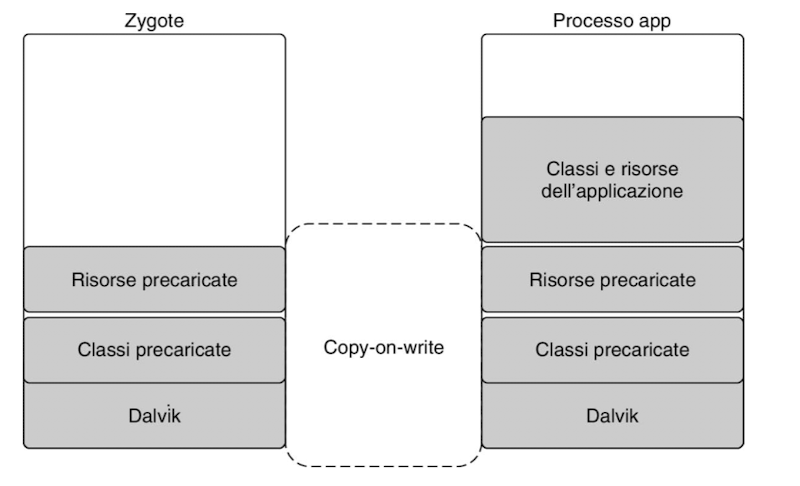
\includegraphics[width=0.5\linewidth]{assets/android-art.png}
\end{figure}

\subsubsection{Binder IPC}
Binder IPC (Inter-Process Communication) è un meccanismo di comunicazione tra processi, utilizzato per permettere lo scambio di dati tra diverse applicazioni e servizi in esecuzione su un dispositivo.

Il Binder opera come un driver nel kernel di Linux, offrendo un'interfaccia ad alte prestazioni per la comunicazione tra processi.

\spacer
Il funzionamento del Binder si basa su un modello client-server, dove i processi client inviano richieste ai processi server. Il server elabora la richiesta e invia una risposta al client.

\spacer
Una delle caratteristiche chiave del Binder IPC è la sua capacità di trasportare riferimenti a oggetti tra processi, mantenendo la sicurezza e l'integrità dei dati.

\spacer
Esso gestisce anche i permessi e l'autenticazione, assicurando che solo i processi autorizzati possano comunicare tra loro. Questo è essenziale per la sicurezza del sistema, specialmente in un ambiente mobile dove molte applicazioni potrebbero provenire da fonti non fidate.

\spacer
Android utilizza il Binder IPC per numerose operazioni interne, come la comunicazione tra i servizi di sistema e le applicazioni. Questo approccio centralizzato permette un controllo rigoroso sulla gestione delle risorse e migliora la stabilità del sistema.

\subsubsection{Applicazioni Android}
Un'applicazione android non è un file eseguibile, ma un contenitore di tutto ciò che costituisce l'app.

I contenuti fondamentali sono:
\begin{sitemize}
    \item Un manifesto che contiene: cos'è l'applicazione, cosa fa e come deve essere eseguita
    \item Le risorse
    \item Il codice
    \item Informazioni sulla firma digitale
\end{sitemize}

\spacer
Non viene fornito un'unico punto di ingresso all'applicazione, ma essi si dividono in:
\begin{sitemize}
    \item \textbf{Attività:} Una parte dell'applicazione che interagisce direttamente con l'utente, il punto principale di accesso all'app.
    \item \textbf{Ricezione:} È un destinatario di eventi, quando il sistema operativo vuole inviare un evento lo fa ad ogni ricevitore installato.
    \item \textbf{Servizio:} I quali possono avere due sfumature:
    \begin{sitemize}
        \item Un'attività di background mantenuta per un lungo tempo.
        \item Un punto di connessione per altre applicazioni.
    \end{sitemize}
    \item \textbf{Fornitura Contenuti:} Il principale strumento utilizzato per lo scambio di dati tra diverse applicazioni. Fornisce un'API alla quale altre applicazioni possono fare richieste e ottenere risposte.
\end{sitemize}

\subsubsection{Sicurezza}
In Android la sicurezza viene implementata con un metodo di minimi permessi. Un'applicazione non ha accesso a nessun dato sensibile se non approvato esplicitamente dall'utente.
